% Turning example: finishing path (blocks N31-N44), upper half section
\documentclass[dvisvgm,tikz,border=4pt]{standalone}
% Shared preamble for the TikZ figures in images-1/src (compiled by build.sh)
\usepackage{helvet}
\renewcommand\familydefault{\sfdefault}
\usepackage{amsmath, amssymb}
\usetikzlibrary{arrows.meta, calc, decorations.pathreplacing, patterns, positioning, shapes.geometric, 3d, perspective, fit, backgrounds}
% palette shared with slides.scss and the Graphviz diagrams
\definecolor{dmred}{HTML}{880000}
\definecolor{dmblue}{HTML}{000088}
\definecolor{dmgreen}{HTML}{008800}
\definecolor{dmorange}{HTML}{E08A1E}
\definecolor{ink}{HTML}{333333}
\definecolor{fillblue}{HTML}{E8E8F8}
\definecolor{fillred}{HTML}{F3EAEA}
\definecolor{fillgreen}{HTML}{E8F4E8}
\definecolor{fillorange}{HTML}{FDF0DC}
\definecolor{steel}{HTML}{C9D3DC}
\definecolor{steeldk}{HTML}{8FA3B5}
\definecolor{metal}{HTML}{D9D9D9}
\definecolor{metaldk}{HTML}{A6A6A6}
\tikzset{
  >={Stealth[length=7pt]},
  every picture/.style={line cap=round, line join=round, font=\large},
  proj/.style={gray, dashed, thin},
  dim/.style={<->, >={Stealth[length=5pt]}, thin},
  ext/.style={very thin, gray},
  callout/.style={gray!70!black, thin},
  % datum (origin) symbol
  % pics use absolute sizes so they look the same in mm-scaled drawings
  datum/.pic={
    \fill[white] (0,0) circle (0.22cm);
    \fill[black] (0,0) -- ++(0.22cm,0) arc[start angle=0, end angle=-90, radius=0.22cm] -- cycle;
    \fill[black] (0,0) -- ++(-0.22cm,0) arc[start angle=180, end angle=90, radius=0.22cm] -- cycle;
    \draw[thick] (0,0) circle (0.22cm);
  },
  % reference symbols (absolute sizes): origins have a double circle with a filled quadrant
  wporigin/.pic={
    \draw[thick, fill=white] (0,0) circle (0.3cm);
    \fill[black] (0,0) -- (0.18cm,0) arc[start angle=0, end angle=-90, radius=0.18cm] -- cycle;
    \draw[thick] (0,0) circle (0.18cm);
    \draw (-0.3cm,0) -- (0.3cm,0) (0,-0.3cm) -- (0,0.3cm);
  },
  machorigin/.pic={
    \draw[thick, fill=white] (0,0) circle (0.3cm);
    \fill[black] (0,0) -- (-0.18cm,0) arc[start angle=180, end angle=90, radius=0.18cm] -- cycle;
    \draw[thick] (0,0) circle (0.18cm);
    \draw (-0.3cm,0) -- (0.3cm,0) (0,-0.3cm) -- (0,0.3cm);
  },
  supportpt/.pic={
    \draw[thick, fill=white] (0,0) circle (0.15cm);
    \draw (-0.15cm,0) -- (0.15cm,0) (0,-0.15cm) -- (0,0.15cm);
  },
  regpt/.pic={
    \draw[thick, fill=white] (0,0) circle (0.24cm);
    \draw[thick] (0,0) circle (0.15cm);
    \draw (-0.15cm,0) -- (0.15cm,0) (0,-0.15cm) -- (0,0.15cm);
  },
  % support / registration point (generic)
  target/.pic={
    \draw[thick, fill=white] (0,0) circle (0.12cm);
    \draw (-0.2cm,0) -- (0.2cm,0) (0,-0.2cm) -- (0,0.2cm);
  },
}

% Turning example (not compiled on its own). Coordinates in mm: x = Z axis, y = radius.
% Profile of the finished part, upper half, from the G-code of the finishing pass.
\newcommand\partprofile{(0,0) -- (0,15) -- (-20,15) -- (-25,12.5) -- (-52,12.5)
  arc[start angle=-90, end angle=-180, x radius=10, y radius=10] -- (-85,22.5)
  -- (-100,32.5) -- (-150,32.5) -- (-150,0)}
% same profile mirrored about the axis (lower half)
\newcommand\partprofilelow{(0,0) -- (0,-15) -- (-20,-15) -- (-25,-12.5) -- (-52,-12.5)
  arc[start angle=90, end angle=180, x radius=10, y radius=10] -- (-85,-22.5)
  -- (-100,-32.5) -- (-150,-32.5) -- (-150,0)}
% roughing passes: (radius, Z end) from blocks N11, N15, N19, N23 (X is a diameter)
\def\roughpasses{30.5/-94.5, 25.5/-88, 20.5/-59.4, 16/-57.6}
\tikzset{mm/.style={x=0.06cm, y=0.06cm}}
% chuck: body and jaws gripping the outer diameter of the stock (radius 32.5) near Z = -150
\newcommand\chuck{%
  \filldraw[thick, fill=metaldk!40] (-182,-54) rectangle (-168,54);
  \foreach \s in {1,-1}
    \filldraw[thick, fill=metaldk!70] (-168,{\s*32.5}) rectangle (-138,{\s*48});}

\begin{document}
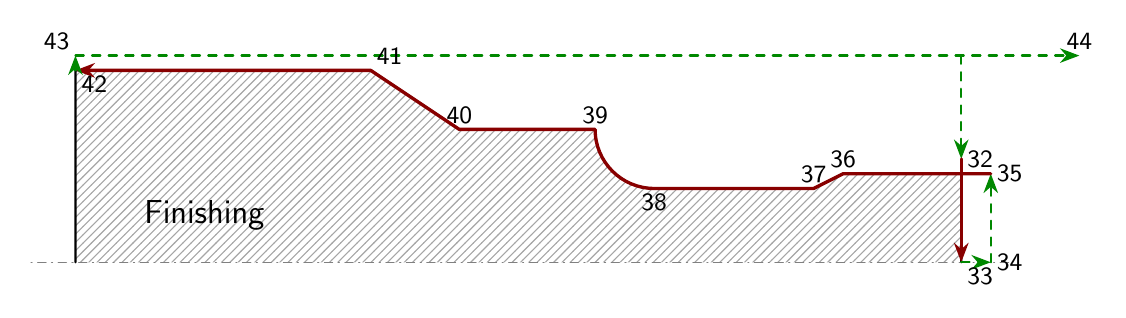
\begin{tikzpicture}[mm, x=0.075cm, y=0.075cm, font=\large]
  \fill[pattern=north east lines, pattern color=gray!70] \partprofile -- cycle;
  \draw[thick] \partprofile;
  \draw[dash dot, gray] (8,0) -- (-158,0);
  \tikzset{rapid/.style={dmgreen, thick, dashed, ->}, feed/.style={dmred, very thick, ->}}
  % G00 rapids dashed, G01/G02 feeds solid; coordinates: (Z, X/2)
  \draw[rapid] (0,35) -- (0,17.5);                                   % N32
  \draw[feed] (0,17.5) -- (0,0);                                      % N33 facing
  \draw[rapid] (0,0) -- (5,0);                                        % N34
  \draw[rapid] (5,0) -- (5,15);                                       % N35
  \draw[feed] (5,15) -- (-20,15) -- (-25,12.5) -- (-52,12.5)          % N36-N38
    arc[start angle=-90, end angle=-180, x radius=10, y radius=10]    % N39 G02
    -- (-85,22.5) -- (-100,32.5) -- (-150,32.5);                      % N40-N42
  \draw[rapid] (-150,32.5) -- (-150,35);                              % N43
  \draw[rapid] (-150,35) -- (20,35);                                  % N44
  % block numbers at the end of each block
  \foreach \p/\n/\a in {{(0,17.5)}/32/right, {(0,0)}/33/below right, {(5,0)}/34/right, {(5,15)}/35/right,
                        {(-20,15)}/36/above, {(-25,12.5)}/37/above, {(-52,12.5)}/38/below,
                        {(-62,22.5)}/39/above, {(-85,22.5)}/40/above, {(-100,32.5)}/41/above right,
                        {(-150,32.5)}/42/below right, {(-150,35)}/43/above left, {(20,35)}/44/above}
    \node[font=\small, \a, inner sep=2pt] at \p {\n};
  \node[anchor=west] at (-140,8) {Finishing};
\end{tikzpicture}
\end{document}
